\section{Thursday, April 20th}
\subsection{Future Interfaces: Virtual and Augmented Reality}
VR has been around since the 1950s with Heilig's Sensorama.

\subsubsection{Changes to costs of VR Hardware}
However VR Arcade Games in the 1990s costed tens of thousands of dollars -- but improved technology are much cheaper now (in the hundreds of dollars or less).

\begin{important}
If the costs are not low enough, some usages of technology will not be discovered. This is yet another reason why making sure hardware is accessible is important.
\end{important}
The most obvious example of the above statement is if you want to be able to draw with brushstrokes in 3D. Would you pay \$20,000 for that? Now what if it is $\approx\$0$, then would you consider using it?

\subsection{Augmented Reality}
Definition:
\begin{shaded}
\textbf{AR} is a computer technology that augments a physical, real-world environment directly or through its indirect view with computer-generated information, including graphics, video, and sound.

AR may alter a user’s view of reality, and may also enhance one’s perception of reality.
\end{shaded}

Note that just like VR, there was a wave of AR in the '90s. The thought was that it'd see usage in car repairs/maintenance among other applications.

Microsoft Hololens2 (2019) showcases this amongst other applications (primarily in games).

\subsubsection{Video see-through AR}
Pokemon Go is the most well-known example of this. \textit{But} it did not really try to understand the scene -- it just placed a Pokemon somewhere even if it's not a realistic horizontal surface or sensible with the current lighting.

\subsubsection{HMD-based AR}
Head Mounted Display is when you have a virtual display mounted on your head. Sometimes this is paired with actual hardware, which the headset then draws on top off (in real-time), to make a more immersive experience.

\subsubsection{Hardware Complexities}
There are lots of sensors and hardware parts, especially in HMDs.

\subsection{Enabling Technologies/
Open Research}
\begin{itemize}
    \item Near-Eye Displays and Optics
    \item 3D Localization
    \item 3D Content Capturing
    \item New Human-Computer Interfaces
\end{itemize}
\begin{center}
    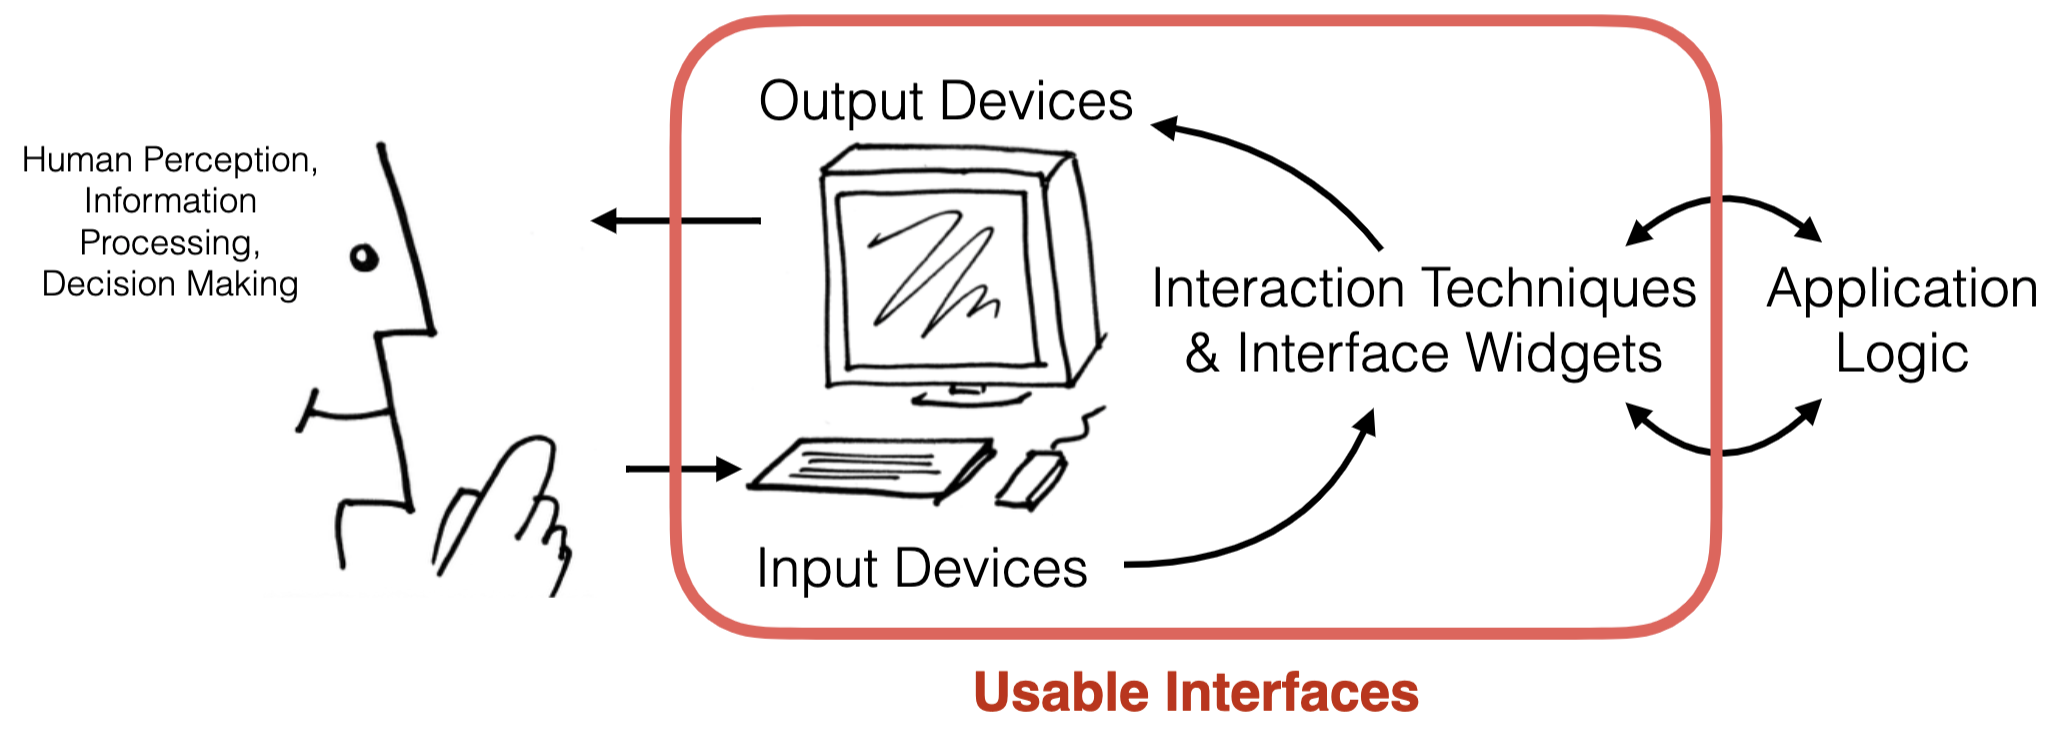
\includegraphics[scale=0.4]{lectures/wk13/img/info_proc_circled.png}
\end{center}

\subsection{Getting Input}
There are 3 important inputs to a VR/AR application: \textbf{Head, Hands and Limbs}.

\subsubsection{3D Glasses}
Red-Blue 3D glasses use light subtraction to make images seem as they come out to you -- but in the process you lose many red and blue colors and get a grayscaling effect.\\
This is known as an Anaglyph (spectral) approach.

However there is also the ``Polarization multiplexing'' approach which is much like polarizing (anti-glare) sunglasses, but with a polarizing filter on each projector.

\subsubsection{Active Shutter}
These were also glasses you could wear to see 3D video from your TV -- these were popular 10-14 years ago.

\subsection{Head-Worn Displays}
These should allow seeing-through so that you can be aware of your environment.

\subsection{Audio Displays}
\subsubsection{Auditory Cues}
\begin{itemize}
    \item Localization: psychoacoustic process of determining direction and location from
which sound emanates
\item Binaural cues:
  \begin{itemize}
    \item ITD interaural time difference
    \item IIT - interaural intensity difference
    \item HRTF - head related transfer function (physical shape of ears, ear canals)
    \item Reverberation
    \item Intensity
  \end{itemize}
\end{itemize}

\[
I \propto \frac{1}{r^2}
\]
where $I$ is the sound pressure level, and $r$ is distance.

HRTF measurement: For far objects, radius less
important. Function of sound frequency and
position: azimuth, elevation,
radius.

\subsection{Reverberation}
Early reflection: localization\\
Long tail late reflection: room characterization

\subsection{Haptic Displays}
\begin{itemize}
    \item Simulate the the physical interaction between the user and objects
    \item Encompasses sensations of force, touch, vibration, temperature
\end{itemize}
Core challenge: cues for particular categories are very different from other categories.

\subsection{Gustation and Olfaction
Displays}
\begin{shaded}
Can we simulate smell and taste?
\end{shaded}
Current answer: No.

Sound: Air pressure variations over time (which is 1-dimensional).
Vision: Red-Green-Blue pixels (which are 3-dimensional).

But smells are a much more complicated dimensionality and carrying a backpack with thousands of smells in jars is not really feasible.

With taste, we have a subset spanned by descriptions (such as salty, sour, sweet, etc) but this does not generate a basis.

\subsection{Professor Hartmann's PhD students' work: Pointing \& Selection in 3D}
How do we select stuff that is further away:
\begin{itemize}
    \item Shrink stuff down
    \item Cast a ray into the scene
\end{itemize}
There has been success in making arms that reach out beyond an actual human's reach -- much like Inspector Gadget's mechanical arms.

Remember that since we are doing a \textit{simulation}, we can alter the laws of physics that are written in the code.

Results: you can control multiple bodies at the same time -- with a natural feeling, despite it being an action that can never happen in reality. Cognitive Science has yet to give an answer to why that is.

\subsection{Bi-manual Scaling}
Pinch-to-zoom but with 2 controllers -- allows us to scale the world up or down.
